\documentclass[11pt]{exam}
\usepackage[margin=1in]{geometry}
\pagestyle{plain}
\usepackage{amsmath,amsfonts,amssymb,amsthm,enumerate}
\usepackage{multicol}
\usepackage[]{graphicx}
\usepackage{hyperref}
\usepackage{tikz}
\usepackage{pgfplots}
\usepackage{subfigure}
\usepackage[final]{pdfpages}

\addtolength{\footskip}{2\baselineskip} % to lower the page numbers
\title{\vspace{-0.5in} Math 115 \\ Worksheet Section 2.3}
\date{}


% \theoremstyle{definition}
% \newtheorem{problem}{Problem}
\renewcommand{\questionlabel}{\textbf{Problem~\thequestion.}}
%\printanswers

\begin{document}
\maketitle
\vspace{-0.75in}
\section*{Warm-up questions}

\noindent
If $f'(x)<0$ on an interval, then $f$ is \fillin[decreasing] on that same interval.

\noindent
If $f'(x)>0$ on an interval, then $f$ is \fillin[increasing] on that same interval.

\noindent
If $f$ is constant on an interval, then $f'(x) =$\fillin[\(0\)] for all values of $x$ in that interval.

\noindent
If $f$ is linear on an interval, then $f'(x) =$\fillin[constant] for all values of $x$ in that interval.
\begin{questions}
  \question  Given the graph below of a function $f(x)$, sketch
    $f'(x)$. (Note, this is a window from \(-4 \leq x \leq 4\) and
    \(-4 \leq y \leq 4\)).

    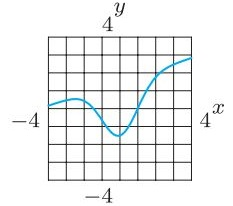
\includegraphics[width=2.8in]{Figures/deriv.jpg}
    \begin{solution}
     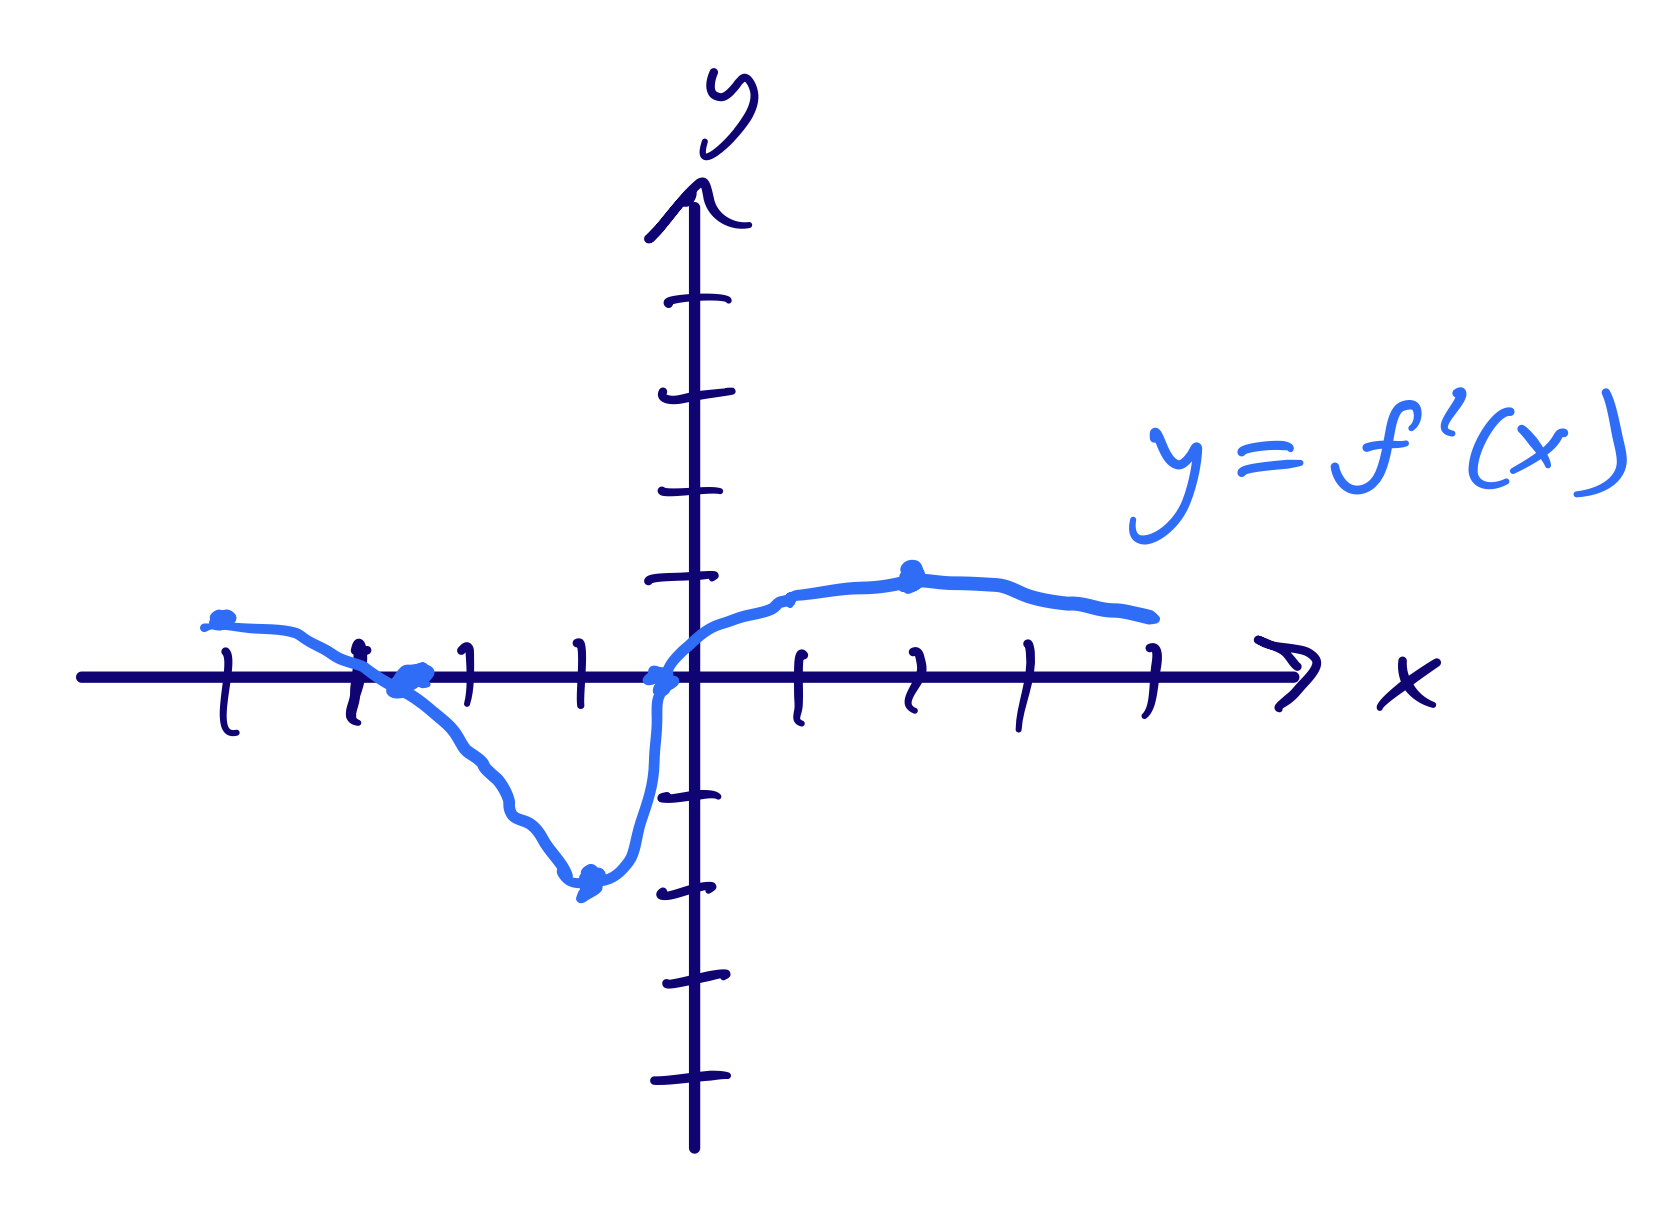
\includegraphics[scale=0.3]{Figures/no1sketch} 
    \end{solution}
  \question One of these graphs is a function $g(x)$ and the other is $g'(x)$.  Which is which?

    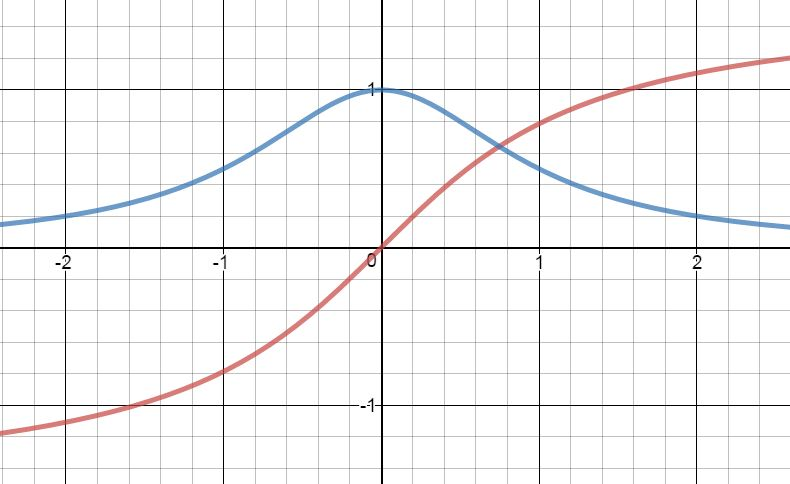
\includegraphics[width=3in]{Figures/arctan.jpg}	

    \begin{solution}
      The red graph is \(y=g(x)\) and the blue graph is
      \(y=g'(x)\). One can check this by noticing that the red graph
      is always increasing, so its derivative has to be entirely
      positive, but the blue graph would have a derivative that starts
      out positive and becomes negative. 
    \end{solution}
  \question Using the table below, estimate $f'(2)$.  Where does $f'(x)$ appear to be positive, negative and zero?  Where does it appear to be largest and smallest?

    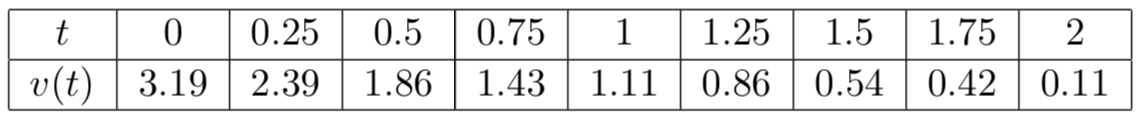
\includegraphics[width=5in]{Figures/table.jpg}	
    \begin{solution}
      \(f'(2) \approx -2\). We can only approximate with the data we
      have, so we can average the slopes of the secant line between
      \((1,f(1))\) and \((2,f(2))\) (which is \(-3\)) and the secant
      line between \((2,f(2))\) and \((3,f(3))\) (which is \(-1\)). 
      \begin{itemize}
      \item \(f'(x)\) appears to be positive on
        \((4,8)\).
      \item \(f'(x)\) appears to be negative on \((0,3)\).
      \item \(f'(x)\) appears to be zero on \((3,4)\).
      \end{itemize}
      \(f'(x)\) appears to be largest between \(7\) and
      \(8\). \(f'(x)\) appears to be smallest between \(0\) and \(1\).
    \end{solution}
  \question Using the limit definition of the derivative, find the
    derivative of \(f(x) = x^2\)
    \begin{solution}
      We check
      \begin{align*}
        f'(x)
        & = \lim_{h \to 0} \frac{f(x+h)-f(x)}{h}\\
        & = \lim_{h \to 0} \frac{(x+h)^2-x^2}{h}\\
        & = \lim_{h \to 0} \frac{x^2+2hx+h^2-x^2}{h}\\
        & = \lim_{h \to 0} \frac{2hx+h^2}{h}\\
        & = \lim_{h \to 0} 2x+h\\
        & = 2x
      \end{align*}
    \end{solution}
  \question \, \\
    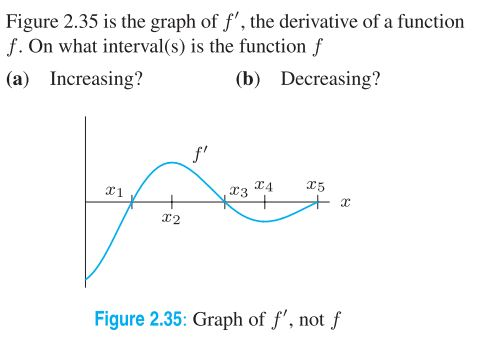
\includegraphics[width=4in]{Figures/no43.jpg}
    \begin{solution}
      \(f\) is increasing wherever \(f'(x) > 0\). This is on
      \((x_1,x_3)\). \(f\) is decreasing wherever \(f'(x) < 0\). This
      is on \((0,x_1)\) and \((x_3,x_5)\).
    \end{solution}
  \question Draw a graph of a continuous function $f(x)$ with
	\begin{itemize}
		\item $f'(x)>0$ for $1<x<3$,
		\item $f'(x)<0$ for $x<1$ and $x>3$ and
		\item $f'(x)=0$ at $x=1$ and $x=3$.
	\end{itemize}
        \begin{solution}
         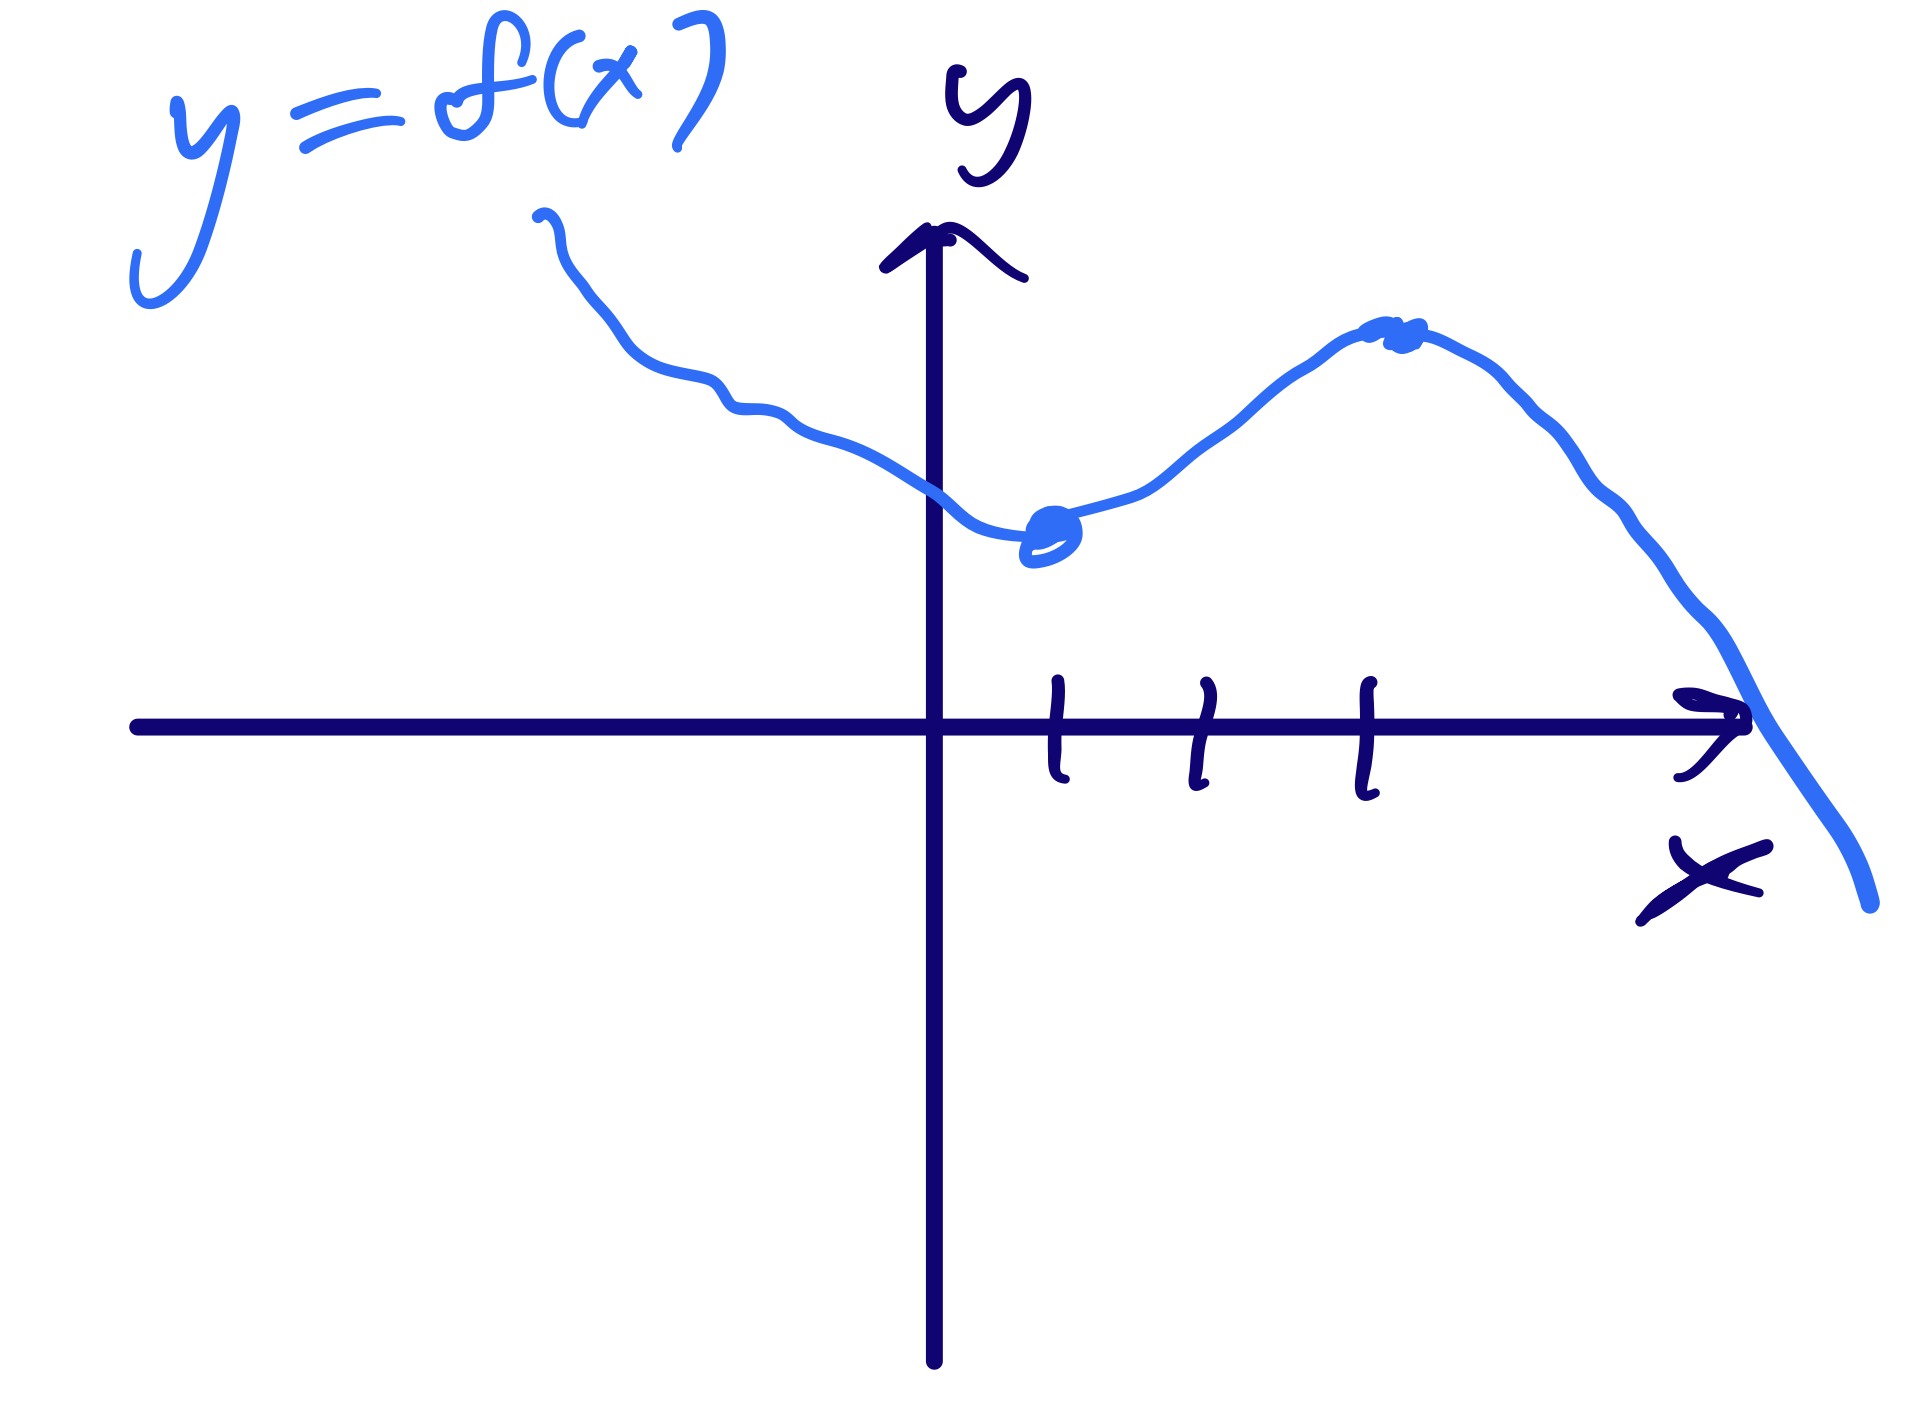
\includegraphics[scale=0.3]{Figures/no6sketch}
        \end{solution}
  \question (Winter 2013 Exam 1) Below is the graph of a function $h$.
\begin{figure}[h]
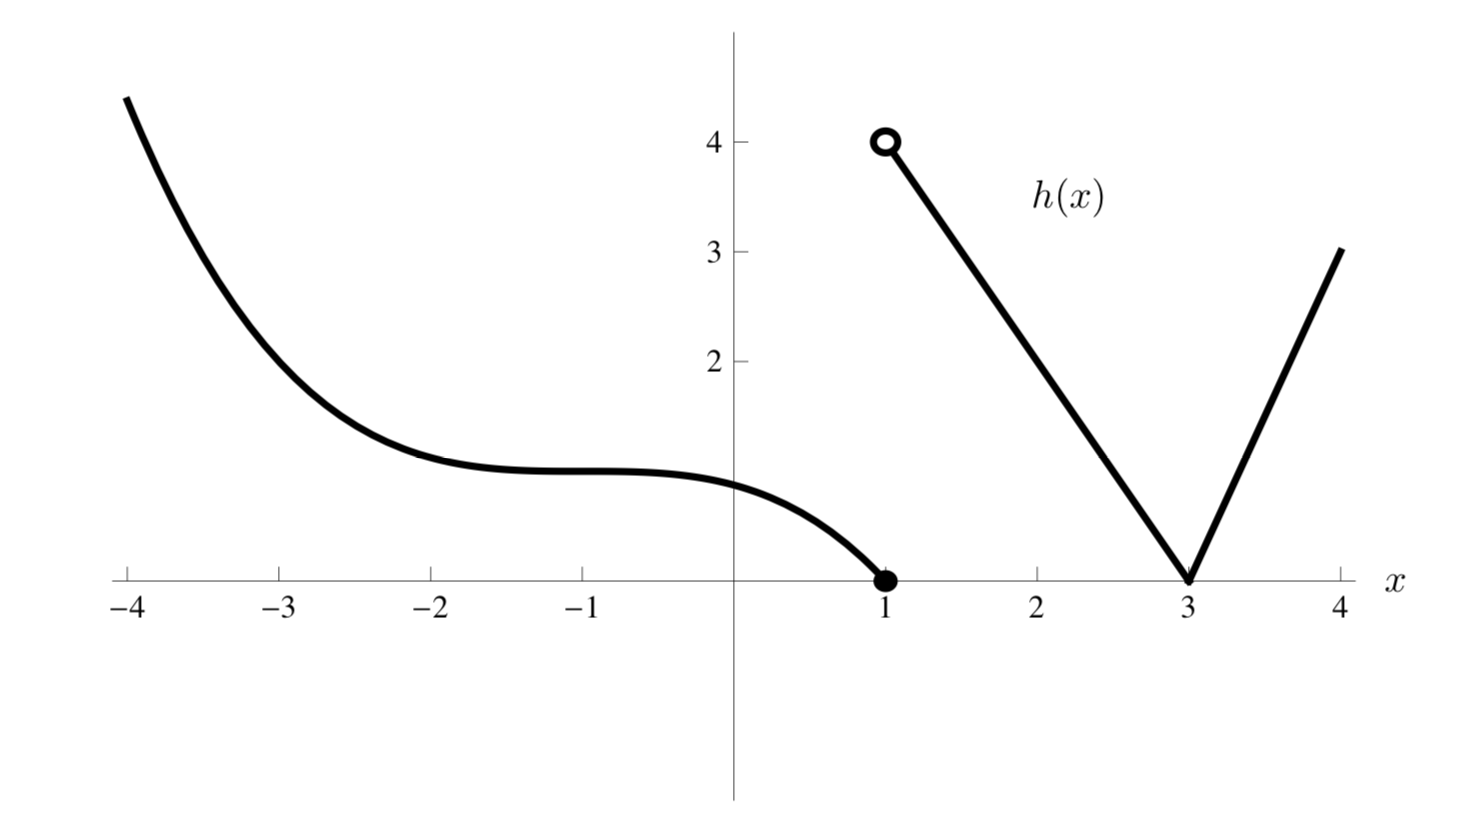
\includegraphics[scale=0.5]{Figures/graphh}
\end{figure}

Carefully draw a graph of $h'(x)$. Be sure to label important points or features on your graph.
\begin{solution}
  See part (c)  of \href{https://dhsp.math.lsa.umich.edu/exams/115exam1/w13/s8.pdf}{https://dhsp.math.lsa.umich.edu/exams/115exam1/w13/s8.pdf}
\end{solution}
\pagebreak
\question (Fall 2009 Exam 1)  If $f(x) = \frac{g(x)}{h(x)}$ and $h(3)=0$, which of the following statements MUST be true?
\begin{enumerate}[(a)]
\item The graph of $f$ has a vertical asymptote at $x=3$.
\item $3$ is not in the domain of $f$.
\item $f$ is not continuous on $[-2,2]$.
\item $\displaystyle\lim_{x \rightarrow 3} f(x)$ does not exist.
\end{enumerate}
\begin{solution}
 (b) \(3\) is not in the domain of \(f\).
\end{solution}
\question (Winter 2013 Exam 1) The figure shows the graph a function $k(x)$ and its tangent line at a point $(a, 2)$. The average rate of change of $k(x)$ between $x = a$ and $x = 6$ is $\frac{1}{6}$.
Find exact numerical values for the following. If it is not possible to find a value, write {\bf NP}.
\begin{figure}[h]
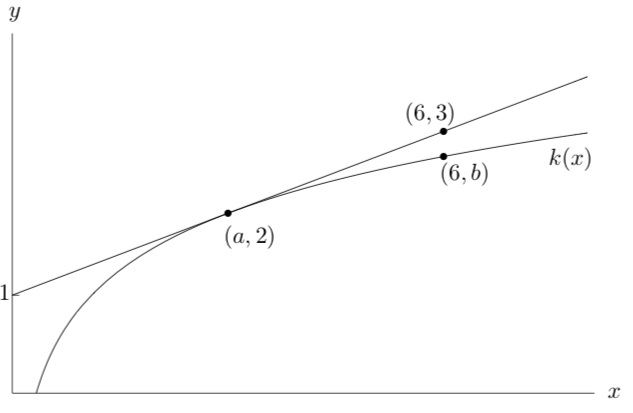
\includegraphics[scale=0.5]{Figures/graphk}
\end{figure}
\begin{multicols}{3}
\begin{enumerate}[(a)]
\item $a =$
\item $b = $
\item $k'(2)=$
\item $k'(a)=$
\item $k'(6)=$
\end{enumerate}
\end{multicols}
\begin{solution}
 See \href{https://dhsp.math.lsa.umich.edu/exams/115exam1/w13/s5.pdf}{https://dhsp.math.lsa.umich.edu/exams/115exam1/w13/s5.pdf}
\end{solution}
\question (Fall 2017 Exam 1) On the board, sketch the graph of a function $y = R(x)$ verifying all of the following conditions:

\begin{itemize}
\item The function $R(x)$ is defined on $-8 \leqslant x \leqslant 9$.
\item $R'(x) = 2$ for $-8 < x < -5$.
\item $R(x)$ is concave down and decreasing on $-5<x<-2$.
\item $R(-2) = 1$.
\item $R(x) = R(-x)$ for $-2 \leqslant x \leqslant 2$.
\item The vertical intercept of $R(x)$ is $y=3$.
\item $\displaystyle\lim_{x \rightarrow 5^-}  R(x) = -2$ but $\displaystyle\lim_{x \rightarrow 5^+} R(x)$ does not exist.
\item $R(x)$ is not continuous at $x=7$ but $\displaystyle\lim_{x \rightarrow 7} R(x)$ exists.
\end{itemize}
\emph{Make sure that your graph is large and unambiguous.}
\begin{solution}
  See \href{https://dhsp.math.lsa.umich.edu/exams/115exam1/f17/s6.pdf}{https://dhsp.math.lsa.umich.edu/exams/115exam1/f17/s6.pdf}
\end{solution}
\question (Winter 2013 Exam 1) In each of the following problems, give a formula for a function whose domain is all real numbers, with all of the indicated properties. If there is no such function, then write “NO SUCH FUNCTION EXISTS”. You do not need to show your work.

\begin{enumerate}[(a)]
\item A sinusoidal function $P(t)$ with the following three properties:
\begin{itemize}
\item The period of the graph of $P(t)$ is 7.
\item The graph of $P(t)$ attains a maximum value at the point $(1, 20)$.
\item The graph of $P(t)$ attains a minimum value at the point $(-2.5,6)$.
\end{itemize}
\item A function $h(x)$ with the following two properties:
\begin{itemize}
\item $h(x)$ is concave down for all $x$.
\item $h(x)>0$ for all $x$.
\end{itemize}
\item A function $j(x)$ with the following two properties:
\begin{itemize}
\item $j(x)$ is decreasing for all $x$.
\item $j(x)$ is concave up for all $x$.
\end{itemize}
\item A rational function $l(x)$ with the following two properties:
\begin{itemize}
\item $l(0)=2$.
\item The line $y = 2$ is a horizontal asymptote to the graph of $l(x)$.
\end{itemize}
\end{enumerate}
\begin{solution}
  See \href{https://dhsp.math.lsa.umich.edu/exams/115exam1/w13/s7.pdf}{https://dhsp.math.lsa.umich.edu/exams/115exam1/w13/s7.pdf} 
\end{solution}
\end{questions}
\end{document}
%%% Local Variables:
%%% mode: latex
%%% TeX-master: t
%%% End:
